\section{Hierarchically Fused Fully Convolutional Network}
\label{Sec:HF-FCN}
In this section, we introduce a novel operation for feature fusion, named hierarchical fusion operation and apply it to the common networks, VGG16 Net and ResNet. The overview diagram in Fig.~\ref{fig:Fusion-Operation} shows where the fusion operations take effect and how they work. Different from other networks for semantic segmentation, we apply the fusion operation twice to integrate information gradually.
Our network consists of three parts. Part 1 is a backbone network whose role is to extract the features at different levels.
In theory, arbitrary feature extraction network is applicable to the Part 1.
The second part is a process of feature fusion in the first stage, which fuses the feature maps generated from each convolutional(conv) layer.
Besides, Part 3 is feature fusion in the second stage.
In the second stage of the fusion process, we take full advantage of the information extracted from the second part by learning the connection weights between upsampled feature maps.

\begin{figure}
\centering
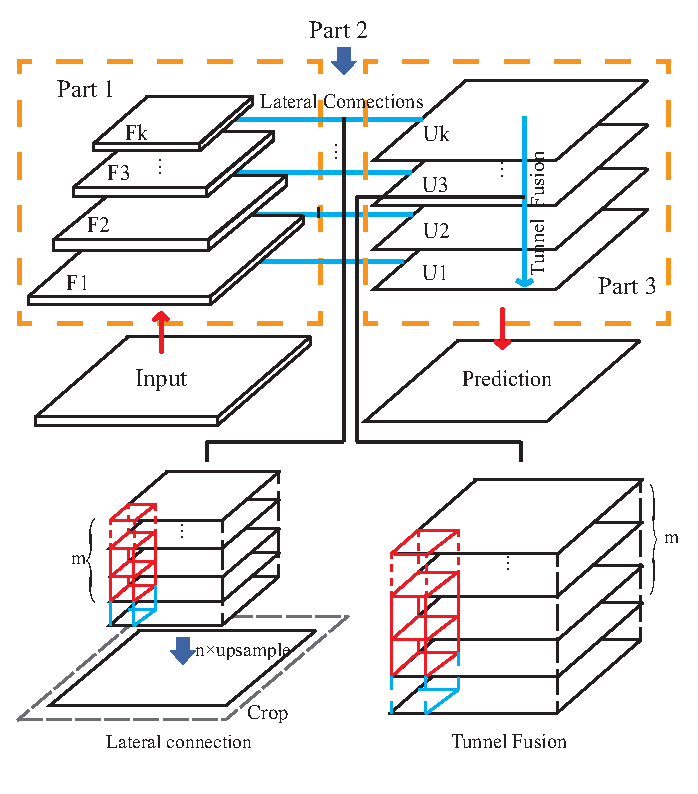
\includegraphics[width=8.5cm]{Figures/Fusion_Operation.eps}
\caption{The first line shows the overview of our network. The second row shows the details of fusion operation. The one on the left is a case where the input is equal to the output and the one on the right is the case of the input not equal to the output.}
\label{fig:Fusion-Operation}
\end{figure}
\cxj{Put overview here. Explain the main components of our methods.}
\subsection{Network Architecture}
 Here, we illustrate our main idea using the VGG16 network as our backbone network, which have been proven to have better performance in experiments.
 Some modifications are made to apply to our building extraction task including removing its fc layers and last pooling layer. The reasons of these changes are
 1) The fc layer generates a fair number of parameters and takes up too much memory.
 2) The existence of fc layer limits the size of input image.
 3) After the last pooling layer, the resolution of the feature map is reduced to 1/32 of the input, which is too small to building extraction task.
 The details of our network using VGG16 Net as backbone network are shown in Fig.~\ref{fig:network_architecture}. The Level 1 in Fig.~\ref{fig:network_architecture} is a trimmed VGG16 Net which regards as our Part 1, backbone network.
 \cxj{Where do you define F1\_1? Is it the layer of VGG16 or HF-FCN?}
 %

In order to leverage the information extracted from different layers, we add the fusion branches on the backbone network.
The branches between Level 1 and Level 2 in Fig.~\ref{fig:network_architecture} form the second part of our network.
The idea is similar to getting the response of scale functions of images when looking for the SIFT feature points. Unlike the feature descriptor of SIFT, we use the concatenated conv layers as our feature extractor.
After getting the responses of different scale functions, the biggest response is selected between adjacent scales of each feature point.
The selecting process is determined by weights learned from fusion operations in our network.
From the perspective of neural networks, the fusion operations in first stage play a role of both feature compression and semantic information fusion in the same levels. They extracts the information from different scales of receptive field as well as diverse levels of semantics.
In addition, the whole weights are learned from the network automatically indicating that network studies the connection relationship among feature maps of same resolution.
\cxj{Fig 1 is the introduction figure.}
With the growing of the receptive field, the detailed information is captured by each conv layer from fine-grained to coarser while the semantic information captured from low level to high level.
For the task of rooftop extraction, not only the details of the appearance of the buildings captured by shallow layers is needed, but also the line and corner extracted by middle layers and the high-level semantics which mainly come from deep layers are needed.
Therefore, we extract various kinds of information by applying the fusion operations to the whole conv layers.
The upsampled feature maps from different conv layers are shown in Fig.~\ref{fig:feature_maps}.
The U1\_1 in Fig.~\ref{fig:feature_maps}(b) means the upsampled feature maps from F1\_1 which are feature maps generated from conv1\_1 with small receptive field extracts low-level features like edges.
In Fig.~\ref{fig:feature_maps}(c), the U1\_2 looks like an over-segmentation which groups pixels with similar color or texture into a subregion.
In the U2\_1, as Fig.~\ref{fig:feature_maps}(d) shows, shape information is augmented.
From the U3\_3, we can see that regions with significantly varying appearance are merged into an integrated building by considering high-level features.
In U4\_3 and U5\_3, more semantic information of rooftop is got, which can distinguish the rooftop and the roads with similar color and deal with the problem caused by shadow.
%

\begin{figure*}
\centering
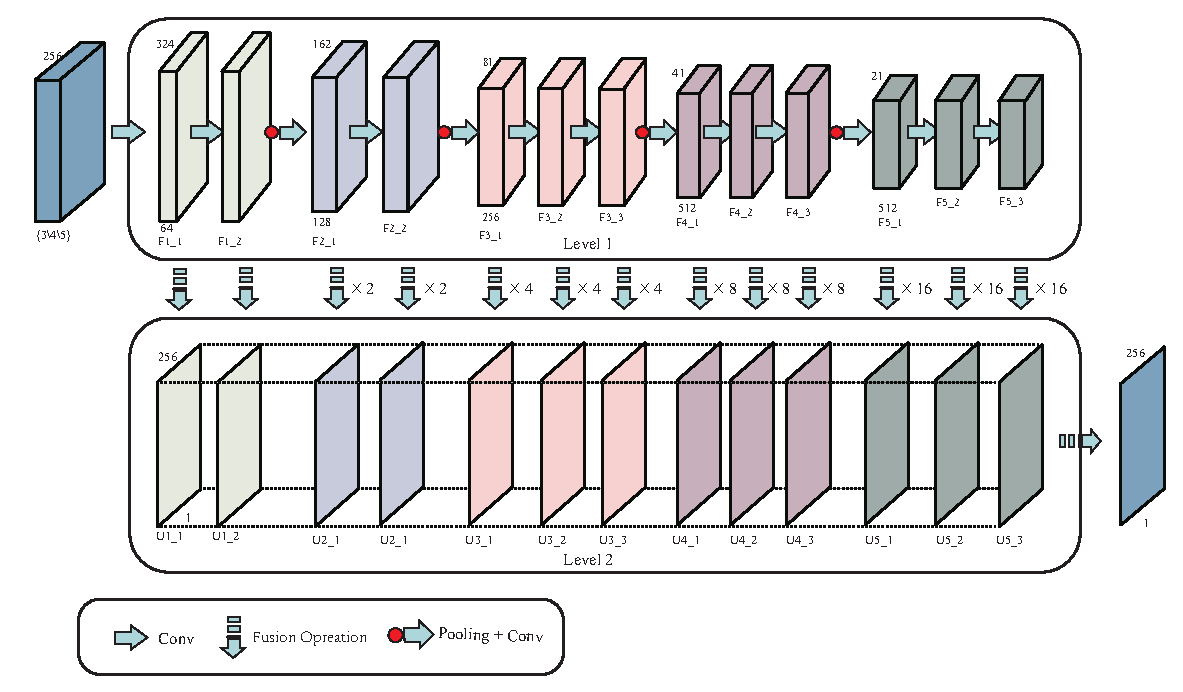
\includegraphics[width=18cm,height=9.5cm]{Figures/network_architecture.eps}
\centering
\caption{Overall architecture of HF-FCN. The input of HF-FCN could be 3, 4 or 5 channels for RGB, DSM, nDSM. The backbone network is VGG16 network which contribute to the Level 1. The F1\_1 in Level 1 indicates the feature maps generated by conv1\_1. In Level 2, 13 upsampled feature maps are cropped to the same size of input. $\times$2 next to the fusion operation means 2 times of upper sampling. U1\_1 in Level 2 means the upsampled feature map of F1\_1, and so forth. \cxj{What is the different between our network with U-Net or other FCN networks?} }
\label{fig:network_architecture}
\end{figure*}

After getting the upsampled feature maps, we fuse them into a final prediction. This is the third part of our network.
Since all the upsampled feature maps are fused, it is expected to achieve a boost in rooftop segmentation which is shown in Fig.~\ref{fig:feature_maps}(h).
In this part, the fusion operation plays a role of feature weighting.
Our intention is learning a group of parameters to combine the upsampled feature maps which is similar to a process of feature selection.
The expression of the formula is as follows:
\begin{equation}
    \label{fature_selection}
    \ y(i,j)=\sum_{n=1}^{N}w_{n}U_{n}(i,j)
\end{equation}
where $y(i,j)$ is a point on the output, ${N}$ is the number of upsampled feature maps and ${U_{n}}$ is a upsampled feature map.


\begin{figure}
\centering
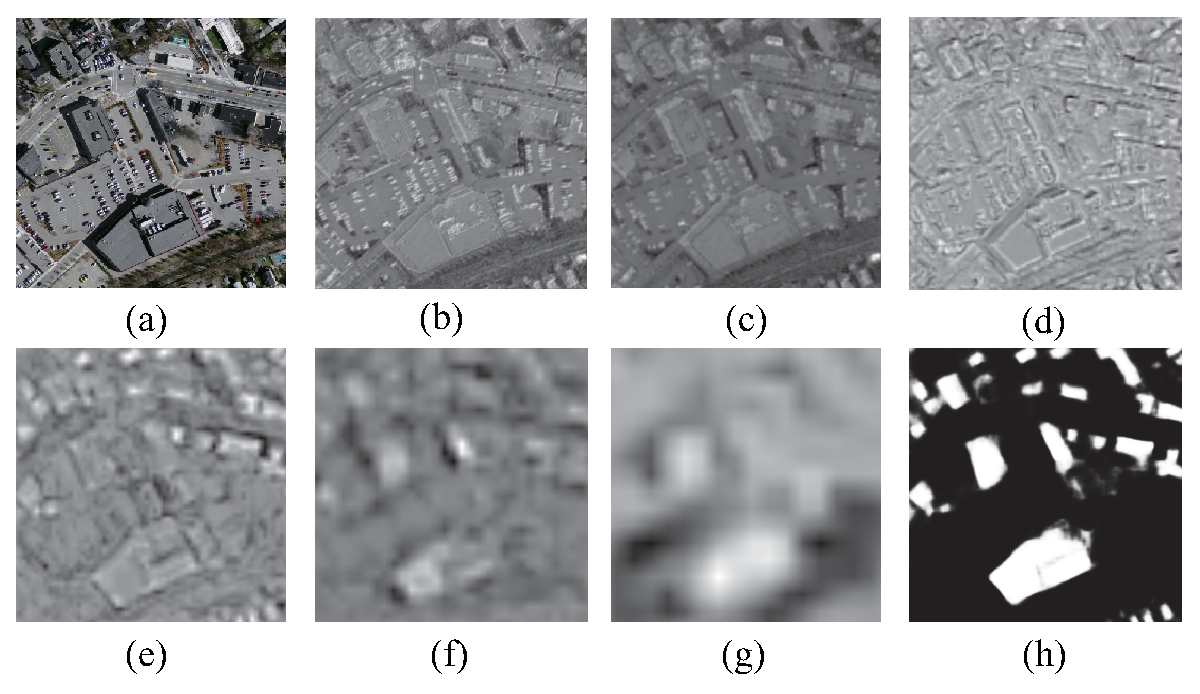
\includegraphics[width=8.7cm]{Figures/feature_maps.eps}
\caption{(a) Input aerial image. (b-g) Feature maps of U1\_1, U1\_2, U2\_2, U3\_3, U4\_3, U5\_3, respectively. (h) Predicted label map.}
\label{fig:feature_maps}
\end{figure}


\subsection{Network Training}

The ground truth $M$ in our dataset is labeled by 0 or 1 to indicate whether a pixel belongs to a roof or not. \cxj{only roof? or part of the building including facades?}
When a remote sensing image ${X}$ is inputted into the network, the output is a prediction probability map $P(X;W)$ of roof, where $W$ denotes all the parameters that learned by HF-FCN. Each pixel value in $P(X_{i};W)$ means the probability of this pixel belongs to rooftop.
We use the sigmoid cross-entropy loss function formulated as
\begin{small}
\begin{equation}
     \label{loss}
     \ L(W)\! =\! -\frac{1}{\vert I\vert}\sum_{i=1}^{\vert I \vert}\lbrack{\tilde{m}_i \log{P(X_{i};W)}\!+\!(1\!-\!\tilde{m}_i)\log(1\!-\!P(X_{i};W)}\rbrack,
\end{equation}
\end{small}
where $\tilde{m}_i$ is label of $X_{i}$, ${\vert I\vert}$ is the number of pixels in the input image ${X}$.
